\section{Results}\label{sec:results}

% <<<<<<< HEAD
% This section presents the results of our research. In Section~\ref{sec:ml}, we compare the performance of various machine learning (ML) algorithms in classifying apps from the \fds dataset as either malware or non-malware using our framework, \droidxpflow. In Section~\ref{sec:family-assessment}, we evaluate the performance of our approach, focusing on malware families and assessing the accuracy of detecting each of them. Finally, in Section~\ref{sec:new-mas-approach}, we provide an overview of the results obtained with our approach and compare them to existing state-of-the-art method.
% =======
This section presents the results of our research. In Section~\ref{sec:ml}, we compare the
performance of machine learning algorithms in classifying as malware or non-malware the
repackaged version of the apps in the \cds dataset, using the network flow data we
collected during the execution of the apps. Recall that previous research employed the \emph{vanilla}
\mas, which relies solely on calls to sensitive APIs for app classification. Our previous
research showed that the performance of the vanilla \mas is compromised when considering
the \cds, in particular due to samples from specific malware families {\color{red}(such as ABC)~\cite{}}.
In Section~\ref{sec:new-mas-approach}, we present the gains in classification performance of our extended \mas,
which combines the analysis of sensitive API calls with our designed network flow ML-based classification method.
Finally, in Section~\ref{sec:family-assessment}, we present assessments of our extended
version of the \mas that focus on the malware families responsible for the poor performance of
the vanilla \mas on the \cds.

\subsection{Comparison of Machine Learning Algorithms}\label{sec:ml}

As discussed in Section~\ref{sec:dataset}, we developed a framework (\droidxpflow), extending DroidXP benchmark to collect network flow information from apps during their execution via DroidBot campaigns. We then conducted our experiment using \droidxpflow, which incorporates network flow data analysis and ML algorithms.

As a first step, we conducted an experiment to compare the performance of various ML algorithms using our \fds dataset for malware classification. This stage of our research considered the following standard ML algorithms:

\begin{itemize}
 \item Logistic Regression (LR)
 \item Linear Discriminant Analysis (LDA)
 \item Quadratic Discriminant Analysis (QDA)
 \item Random Forest (RF)
\end{itemize}

We also explored the Energy-Based Flow Classifier (EFC), which has been used for intrusion and botnet detection using network flows~\cite{DBLP:journals/tnsm/PontesSGBM21}. For our experiments with \fds, $70\%$ of the samples ($2,847$) were allocated for training, and $30\%$ ($1,220$ samples) for testing. To maximize the performance of each ML algorithm, we explored multiple parameter configurations, using cross-validation, to making efficient use of the available features for each ML algorithm.

Ultimately, the RF algorithm outperformed the others when evaluated with standard metrics (recall, precision, F1-score, and Area Under the Curve (AUC)). Table~\ref{tab:ml-metrics} presents the results. Thus, based on these findings, we answer the research questions using the outputs of the RF algorithm classification.



\begin{table}[htb]
    \caption{Accuracy of the ML algorithms to classify the app as malware or non-malware using network flow data from the \fds.}
  \begin{tabular}{lcccc} \toprule
    Algorithm & Precision & Recall & \fone & AUC \\ \midrule 
    LR  & 0.74 & 0.98 & 0.84 & 0.74 \\
    LDA & 0.74 & 0.97 & 0.84 & 0.84 \\
    QDA & 0.72 & 0.66 & 0.69 & 0.76 \\
    EFC & 0.75 & 0.97 & 0.85 & 0.66 \\
    RF & 0.87 & 0.90 & 0.89 & 0.94 \\ \bottomrule    
  \end{tabular}
  \label{tab:ml-metrics}
\end{table}

\begin{finding}
  The RF algorithm outperforms the others popular classification algorithms, achieving higher values across the metrics explored (recall, precision, \fone, and Area Under the Curve).
\end{finding}


% \begin{figure*}[h]
%   \centering  
%     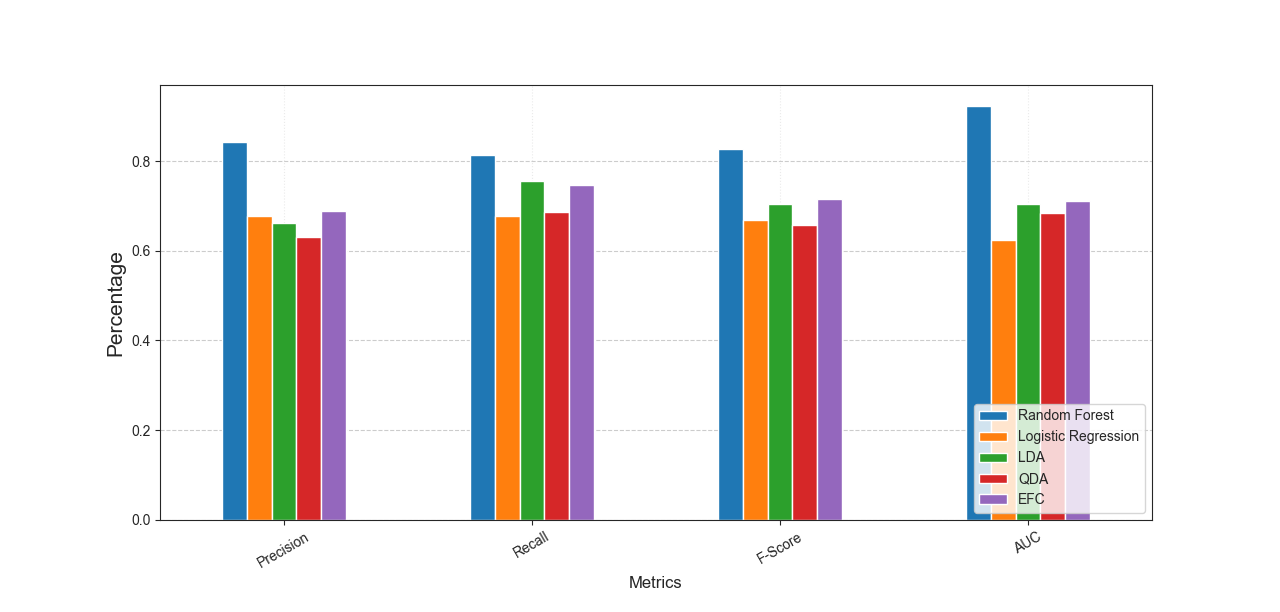
\includegraphics[width=0.85\textwidth]{image/barGraphMetrics.png} \\[\abovecaptionskip]
%   \caption{The comparison of machine learning algorithms}\label{fig:metrics}
% \end{figure*}

\subsection{Detection Performance based on Malware Family}\label{sec:family-assessment}

In this section, we present the performance of our experiment based on malware family. Since the number of samples in each family varies, the overall detection rate is more influenced by families with larger sample sizes. However, our results become inconsistent if we use the same number of samples for each family. To resolve this issue, we present the results based on the actual number of samples from the $20$ most representative families, which account for $90.9\%$ of all malware samples tested and whose families could be labeled by \vt.

We also explored the detection rate of recent malware samples. Although their families are unknown, we demonstrated that it is possible to classify them as suspicious apps using our framework (Section~\ref{sec:unknowfamily}).


\subsubsection{Detection rate of 20 most representative malware families}\label{sec:familyDetection}


Among the $20$ most representative families, the families with the highest earnings are \gps and \dwg. Among the $69$ samples evaluated from the \dwg family, \droidxpflow flagged $66$ apps ($95.65\%$) as malicious. Despite this, the \dwg family does not have as many representative samples as the \gps family, which accounts for $46.96\%$ of all samples tested in the \fds, with $372$ samples. Of these, \droidxpflow flagged $348$ samples ($93.55$\%) as malicious. Malware belonging to the \gps family automatically connects to networks, communicates with remote servers, downloads and installs other apps or adware without the user’s knowledge\cite{DBLP:journals/jnca/WangCYYPJ19}. Due to their high network interaction, they are more easily detected by our framework, demonstrating its effectiveness in detecting samples with malicious network behaviors.

Additionally, it is worth noting that among the $20$ most representative families examined, our framework correctly identified all samples as malware in 12 families. This result demonstrates that our approach is effective for other malware families investigated as well. Table~\ref{tab:families_rate} shows the detection performance of our strategies for the $20$ most representative families. The table also classify samples from five malware categories: ad fraud, adware, spyware, trojans, and SMS malware. Most of the samples are from the adware and ad fraud categories, which aggressively display ads, generate fraudulent ad clicks, and track user behavior~\cite{DBLP:journals/spe/FallahB22}. The other categories are equally harmful and may cause financial losses through unauthorized messages (SMS malware), collect sensitive user data for malicious purposes (Spyware), or provide remote access and control over infected devices (Trojans).



\begin{table*}[h]
  \caption{Detection Rate of the $20$ most representative Families from $30\%$ tested randomly selected from \fds.}
\centering{
  \begin{tabular}{llrrr} \hline
    Category & Family & Samples & Detected  & \%  \\
    \hline

        Ad Fraud & gappusin & 372 & 348 & 93,55  \\
        ~ & dowgin & 69 & 66 & 95,65  \\
        ~ & kyvu & 4 & 4 & 100,00  \\
        Adware & revmob & 67 & 62 & 92,54  \\
        ~ & airpush & 44 & 42 & 95,45  \\
        ~ & youmi & 28 & 28 & 100,00  \\
        ~ & kuguo & 22 & 22 & 100,00  \\
        ~ & leadbolt & 15 & 15 & 100,00  \\
        ~ & adwo & 10 & 10 & 100,00  \\
        ~ & apptrack & 10 & 10 & 100,00  \\
        ~ & domob & 9 & 9 & 100,00  \\
        ~ & appsgeyser & 6 & 5 & 83,33  \\
        ~ & admogo & 6 & 5 & 83,33  \\
        ~ & pircob & 5 & 5 & 100,00  \\
        ~ & cimsci & 4 & 4 & 100,00  \\
        
        ~ & dnotua & 3 & 3 & 100,00  \\
        Spyware & igexin & 7 & 7 & 100,00  \\
        ~ & cnzz & 4 & 4 & 100,00  \\
        Trojan & torjok & 8 & 7 & 87,50  \\
        SMSmalware & smsreg & 29 & 27 & 93,10  \\

   
    \hline
  \end{tabular}
  }
  \label{tab:families_rate}
\end{table*}


\begin{finding}

Our approach proved to be efficient at malware families with high network interaction, like demonstrated at samples from \gps family, the most representative family in \fds. This demonstrates the potential of this solution in detecting samples with malicious network behaviors.

\end{finding}


\subsubsection{Detection rate of unknown malware family}\label{sec:unknowfamily}

According to \vt, among the samples from our \fds, at least two security engines identified $80$ samples as malware, but they were unable to specify their families. Since new malware emerges daily, accurately classifying recent malicious apps into their respective families is both challenging and time-consuming~\cite{DBLP:journals/compsec/WangTW21,DBLP:journals/compsec/ContiKP22}, suggesting that these are recent malware.

Although the specific families were unknown at the time of this research, our framework flagged $39$ samples ($48.75\%$) as malicious. Based on these results, we conclude that \droidxpflow can classify recent apps as malware based solely on their malicious network activity.

\begin{finding}

Even for recently malicious apps without family classification, our approach can flag them as malware based solely on their suspicious network activities.

\end{finding}



\subsection{Flow Analysis approach x Mining Android Sandbox (MAS) approach}\label{sec:new-mas-approach}


In this section, we compare the performance of \droidxpflow and \mas classifier, presented in the previous chapter of this thesis. The comparison is performed based on standard metrics (recall, precision, F1-score). To provide a baseline comparison, we present the results of the \mas using the same $30\%$ of samples ($1,220$) from the \fds dataset tested in section~\ref{sec:ml}.

Our results demonstrate that the vanilla \mas for malware classification has lower performance (\fone) compared to the \droidxpflow framework. In summary, the results reveal that the \mas achieves an \fone of $59\%$, while the \droidxpflow achieves an overall accuracy of $89\%$.

To understand the strengths and weaknesses of each method, we further analyzed their contributions to the \fds dataset. We report the increase in True Positives (TP) and False Positives (FP) for each technique in Figure~\ref{fig:venn}. The figure shows that different approaches contribute differently to the final detection results. More details are provided in the following subsection.


\subsubsection{\mas result} 

Considering $30\%$ of the \fds (1,220 apps), the \mas flagged a total of $460$ repackaged apps as malware ($37.7\%$ of the total number of repackaged apps investigated), where the repackaged app version calls at least one additional sensitive API. We explored accuracy metrics (such as Precision, Recall, and F-measure (F1)), taking advantage of \vt to label the \fds and build a ground truth. Table~\ref{tab:accuracy} summarizes the results of the study (first row).

The results indicate that the \mas achieves an accuracy of $0.59$ when considering the $1,220$ apps explored. Nonetheless, the \mas fails to correctly classify $488$ assets as malware (FN column, first row of Table~\ref{tab:accuracy}) and wrongly labels the repackaged version of $64$ apps as malware (FP column). Therefore, the study reveals a lower performance in terms of accuracy, indicating that when considering $30\%$ of the \fds, the accuracy of the \mas using DroidBot as the test generation tool is nearly $60\%$.


\subsubsection{Flow Analysis result} 

Surprisingly, considering the same samples ($1,220$ apps), we explored our framework. The \droidxpflow labeled a total of $903$ apps as malware but failed to correctly label $86$ assets as malware. However, it wrongly labeled the repackaged versions of $116$ samples as malware (second row of Table~\ref{tab:accuracy}). Our \droidxpflow framework showed better performance compared to the \mas, with an accuracy rate of $89\%$. Based on these results, we can conclude that \droidxpflow outperforms the \mas, proving to be an effective strategy for malware classification. In the next section, we present the strengths and weaknesses of each proposal.


\begin{finding}
The experimental results demonstrate that \droidxpflow framework, outperforms the \mas, with \fone of $0.89$. This proves that the approach is an effective strategy for malware identification.
\end{finding}


\begin{table*}
  \caption{Accuracy of both strategy on \fds (1220 samples).}
\centering{
  \begin{tabular}{lrrrrrr} \hline
    Approach & TP   & FP  & FN  & Precision & Recall & $F_1$ \\
    \hline
    \mas   & 396  & 64 & 488 & 0.86       & 0.45   & 0.59  \\
    Flow Analysis with ML support (RF)    & 787   & 116   & 86   & 0.87      & 0.90   & 0.89  \\
    
    \hline
  \end{tabular}
  }
  \label{tab:accuracy}
\end{table*}


\subsection{Weakness and Strength of \net and \mas}\label{sec:strategy}

To understand the benefits of each method, we further analyze the contribution of both methods in detecting malicious samples. We report the increase in True Positives (TP), False Positives (FP), and False Negatives (FN) for each technique in Figure~\ref{fig:venn}. The figure reveals that different approaches contribute differently to the final detection result.

In the first Venn diagram of Figure~\ref{fig:venn}, we present the increase in True Positives (TP) for our samples. As we can see, $432$ samples were classified solely by \droidxpflow, most of them from the \gps family ($292$ samples). Both approaches detected $358$ samples, most of them from \gps, \fm{airpush}, and \dwg. The \mas correctly detected $30$ samples on its own, most of them without family classification ($14$ samples).

The second Venn diagram presents the increase in False Positives (FP). The diagram shows that the \mas has a lower increase in FP compared to \droidxpflow, which can explain its precision in Table~\ref{tab:accuracy}. \droidxpflow has almost twice as many samples with FP as the \mas. For $97$ benign samples, the approach mistakenly classified a normal network flow as malicious. However, its precision remains high due to the increase in True Positives (TP).

Finally, in the last Venn diagram, we can see the samples that both approaches failed to classify as malicious. The diagram shows that the \mas has a high increase in False Negatives (FN) ($432$ samples), most of them from the \gps family ($292$ samples), which are more easily detected by our framework due to their malicious network behaviors, as presented in Section~\ref{sec:familyDetection}. Among the 56 samples that were not detected by either approach, most of them ($28$) do not have a family classification. According to \vt, among the 60 antivirus engines available, at most 4 are capable of detecting them, characterizing these samples as complex and difficult to classify as malware.


\begin{figure}[t!]
  \centering
  \begin{tabular}{@{}c@{}}
    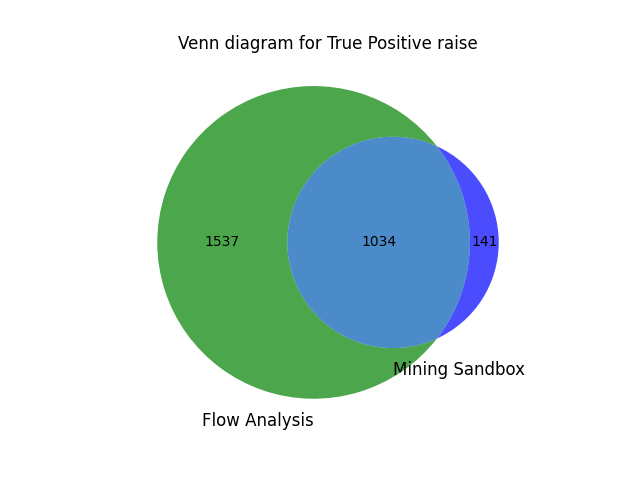
\includegraphics[width=0.5\textwidth]{image/vennTP.png} \\[\abovecaptionskip]
    \small (a) True Positive raise
  \end{tabular}

  \begin{tabular}{@{}c@{}}
    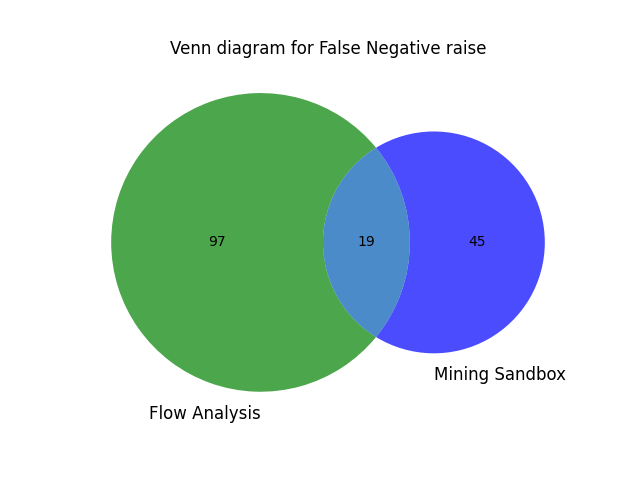
\includegraphics[width=0.5\textwidth]{image/vennFP.png} \\[\abovecaptionskip]
    \small (b) False Positive raise
  \end{tabular}
   \begin{tabular}{@{}c@{}}
    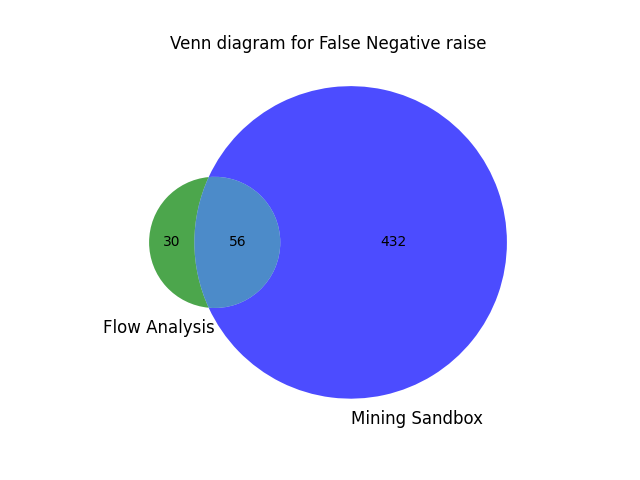
\includegraphics[width=0.5\textwidth]{image/vennFN.png} \\[\abovecaptionskip]
    \small (c) False Negative raise
  \end{tabular}

  \caption{Contribution to the final detection result}\label{fig:venn}
\end{figure}



